\documentclass[12pt, a4paper]{article}
\usepackage[utf8]{inputenc}
\usepackage{amsmath}
\usepackage{amsthm}
\usepackage{graphicx}
\usepackage{parskip}
\usepackage{titling} 
\usepackage{hyperref}
\usepackage{fancyhdr}
\usepackage{lastpage}
\usepackage{listings}
\usepackage{color}
\usepackage{caption}
\usepackage{pgfplots}
\definecolor{dkgreen}{rgb}{0,0.6,0}
\definecolor{gray}{rgb}{0.5,0.5,0.5}
\definecolor{mauve}{rgb}{0.58,0,0.82}

\lstset{frame=tb,
  language=Java,
  aboveskip=3mm,
  belowskip=3mm,
  showstringspaces=false,
  columns=flexible,
  basicstyle={\small\ttfamily},
  numbers=left,
  numberstyle=\tiny\color{gray},
  keywordstyle=\color{blue},
  commentstyle=\color{dkgreen},
  stringstyle=\color{mauve},
  breaklines=true,
  breakatwhitespace=true,
  tabsize=2,
  stepnumber=1,
}

\title{
  Randomized Algorithms\\
  Assignment 1 Fall 2019\\
  UPC - MIRI
}
\author{Juan Pablo Royo Sales - Francesc Roy Campderrós}
\date\today

\pagestyle{fancy}
\fancyhf{}
\fancyhead[C]{}
\fancyhead[R]{Royo Sales - Roy Camperrós}
\fancyhead[L]{UPC - MIRI - RA - Assignment 1}
\fancyfoot[L,C]{}
\fancyfoot[R]{Page \thepage{} of \pageref{LastPage}}
\renewcommand{\headrulewidth}{0.4pt}
\renewcommand{\footrulewidth}{0.4pt}


\graphicspath{ {./images/} }

\begin{document}

\begin{titlingpage}
  \maketitle
\end{titlingpage}

\section{File Organization}

\begin{itemize}
\item \textbf{src}: This is the folder where Source Code can be found.
\item \textbf{docs}: This is the folder where Documentation Latex and images
    can be found.
\item \textbf{samples}: This is the folder where all the $MAX(S_n)$ samples can
  be found.
  \begin{itemize}
    \item On this folder all the samples are organized by $|S_n|$. For
  example on folder \lstinline|samples/m16_sn500| we can found the samples which
  $|S_n| = 500$.
    \item File names are In this case all the files are named with the following
      pattern \lstinline|sample_ITERATION_m_16_SNNUMER| where \textbf{ITERATION}
      is the iteration step which is between 0 and 999 and SNNUMER is $|S_n|$
  \end{itemize}
\end{itemize}

\section{Algorithm explanation}

In order to describe the algorithm we have implemented, the straightforward path
is to begin from the main function that perform all the steps to generate the
Expected value.

\begin{lstlisting}[language=Java,caption={runExperiments function},label={fn:runexp}]
public void runExperiments(){
  Integer[] numberUndominatedStrings = new Integer[experiments];
  for(int i=0;i<experiments;i++){
            
    //Set S_n
    List<String> sn = generateSample();
     // Caluclate MAX(S_n)
    Set<String> maxUndominantSet = maxUndominant(sn);
     try {
        String collect = maxUndominantSet.stream().collect(Collectors.joining("\n"));
        Files.write(Paths.get("./sample_"+i+"_m_"+chainLength+"_sn"+samples+".txt"), collect.getBytes());
    } catch (IOException e) {
        e.printStackTrace();
    }
     // Count all ones chain ocurrence on Max(S_n)
    numberAllOnesString += Collections.frequency(maxUndominantSet, allOnes());
     //Store |MAX(S_n)| as a sample
    numberUndominatedStrings[i]= maxUndominantSet.size();
 }
 expectedValue = getMedian(numberUndominatedStrings);
}
\end{lstlisting}


As we can appreciate in \ref{fn:runexp} we have parameterized every possible
value such as $S_n$, $m$ and the number of iterations, which for the purpose of
the experiment we have set to $1000$ for every experiment run.

The main algorithm which is the ``runExperiments'' function can be described as
the following steps:

\begin{enumerate}
 \item Generate the sample $S_n \mid n << |U| \text{ of } m$

For that purpose we implement a method to u.a.r generate ${1,0}^m$ with $m = 16$
strings using the following for generating bit to bit each string:

\begin{lstlisting}[language=Java,caption={tosCoin function},label={fn:toscoin}]
  private char tosCoin(){
    return (char)(random.nextInt(2)+'0');
  }
\end{lstlisting}


\item Extract the subset $MAX(S_n)$ of undominated strings.
  To achieve this goal we implement a Divide and Conquer algorithm where we
  divide our $S_n$ by 2 recursively until we reach the base case. In each $\beta$
  reduction step after base case is reached, we compare to get the undominated
  chains, reducing the amount of the subset throughout the recursion steps.


\begin{lstlisting}[language=Java,caption={maxUndominant function},label={fn:maxUndominant}]
  public Set<String> maxUndominant(List<String> sn){
    // Base Case: Two or less elements to compare and check dominants between them
    if(sn.size() <= 2){
      Set<String> doms = new HashSet<>();
      compareAndSetDominantForEach(doms, new HashSet<>(sn));
      return doms;
    }


    // Establish medium index to recurse left and right
    int m = sn.size() / 2;
    // Get MAX(Sn) for Left
    Set<String> leftMaxUndominant = maxUndominant(sn.subList(0, m));
    // Get MAX(Sn) for Right
    Set<String> rightMaxUndominant = maxUndominant(sn.subList(m, sn.size()));

    Set<String> dominantsRec = new HashSet<>();
    // Merge left and right dominants subsets and keep non dominant between them
    compareAndSetDominantForEach(dominantsRec, leftMaxUndominant);
    compareAndSetDominantForEach(dominantsRec, rightMaxUndominant);
    return dominantsRec;
  }
\end{lstlisting}

Here \ref{fn:maxUndominant} we can see the Divide and Conquer algorithm
explained before. 

\begin{lstlisting}[language=Java,caption={compareAndSetDominant function},label={fn:compareAndSetDominant}]
  public void compareAndSetDomiant(Set<String> dominants, String elem) {
    Iterator<String> iterator = dominants.iterator();
    boolean addElem = true;
    while(iterator.hasNext()){
      String next = iterator.next();
      if(isDominant(next,elem)) {
        addElem = false;
        break;
      }
      if(isDominant(elem, next)){
        iterator.remove();
      }
    }
    if(dominants.isEmpty() || addElem){
      dominants.add(elem);
    }
  }
\end{lstlisting}

\ref{fn:compareAndSetDominant} is where the merge step
take place, trying to not increment or event reduce the Undominated set for the
next merge recursion step.

\item When recursion is finished, we get $MAX(S_n)$, we store this iteration
  sample and we increment the counter which is registering if this $MAX(S_n)$ is
  a Singleton Set with all one's bits. Recall \ref{fn:runexp} from line 9-16.

\item After running all the experiments, we calculate median to get $E[M_n]$.
  Calculation of the median we do it with a QuickSelect algorithm to have $O(n)$
  cost.

\begin{lstlisting}[language=Java,caption={QuickSelect Algorithm},label={fn:quickselect}]
public class QuickSelect {

    public static <T extends Number> int median(List<T> coll, Comparator<T> comp) {
        int result;
        int n = coll.size()/2;

        if (coll.size() % 2 == 0)  // even number of items; find the middle two and average them
            result = (nth(coll, n-1, comp).intValue() + nth(coll, n, comp).intValue()) / 2;
        else                      // odd number of items; return the one in the middle
            result = nth(coll, n, comp).intValue();

        return result;
    }


    public static <T> T nth(List<T> coll, int n, Comparator<T> comp) {
        T result, pivot;
        List<T> underPivot = new ArrayList<>(), overPivot = new ArrayList<>(), equalPivot = new ArrayList<>();

        // choosing a pivot is a whole topic in itself.
        // this implementation uses the simple strategy of grabbing something from the middle of the ArrayList.

        pivot = coll.get(n/2);

        // split coll into 3 lists based on comparison with the pivot

        for (T obj : coll) {
            int order = comp.compare(obj, pivot);

            if (order < 0)        // obj < pivot
                underPivot.add(obj);
            else if (order > 0)   // obj > pivot
                overPivot.add(obj);
            else                  // obj = pivot
                equalPivot.add(obj);
        } // for each obj in coll

        // recurse on the appropriate list

        if (n < underPivot.size())
            result = nth(underPivot, n, comp);
        else if (n < underPivot.size() + equalPivot.size()) // equal to pivot; just return it
            result = pivot;
        else  // everything in underPivot and equalPivot is too small.  Adjust n accordingly in the recursion.
            result = nth(overPivot, n - underPivot.size() - equalPivot.size(), comp);

        return result;
    }


  }

\end{lstlisting}

\end{enumerate}

\section{Experiments}\label{sec:exp}
We have made some different types experiments always with a value $m = 16$ and 1000 attemps, but changing the value of $|S_n|$

\subsection{$|S_n| = 500$}

\begin{minipage}[t]{\linewidth}
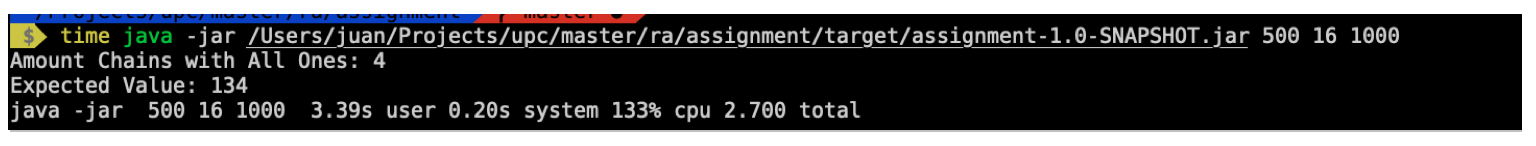
\includegraphics[width=\textwidth]{experiment1}
\captionof{figure}{Experiment with n=500}
\label{fig:experiment1}
\end{minipage}

\subsection{$|S_n| = 1500$}

\begin{minipage}[t]{\linewidth}
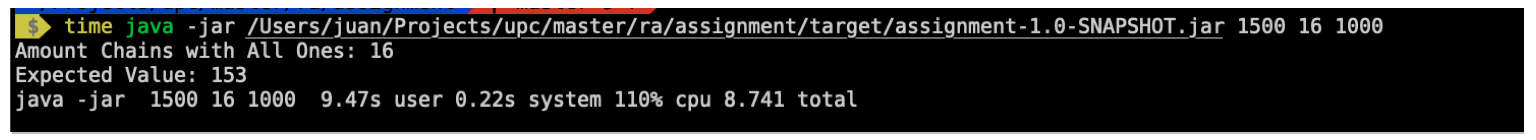
\includegraphics[width=\textwidth]{experiment2}
\captionof{figure}{Expriment with n=1500}
\label{fig:experiment2}
\end{minipage}

\subsection{$|S_n| = 3000$}

\begin{minipage}[t]{\linewidth}
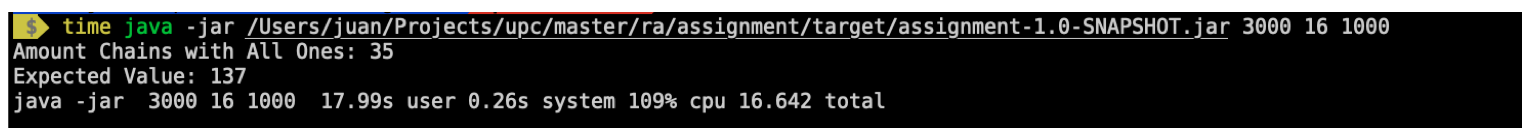
\includegraphics[width=\textwidth]{experiment3}
\captionof{figure}{Expriment with n=3000}
\label{fig:experiment3}
\end{minipage}

\subsection{$|S_n| = 6000$}

\begin{minipage}[t]{\linewidth}
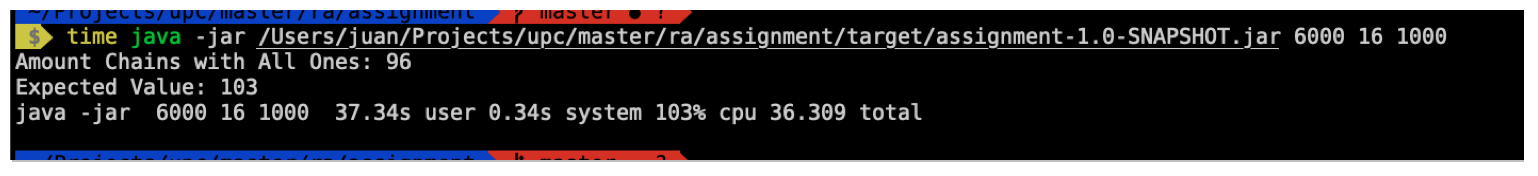
\includegraphics[width=\textwidth]{experiment4}
\captionof{figure}{Expriment with n=6000}
\label{fig:experiment4}
\end{minipage}

\subsection{$|S_n| = 10000$}

\begin{minipage}[t]{\linewidth}
  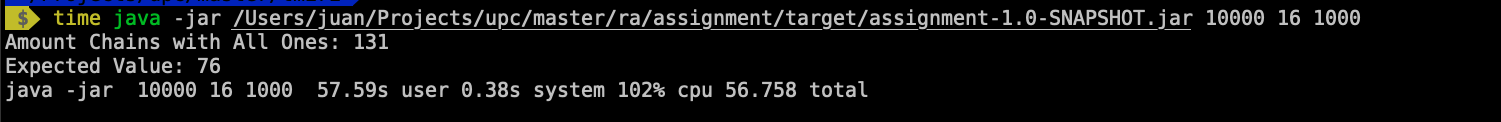
\includegraphics[width=\textwidth]{experiment5}
  \captionof{figure}{Expriment with n=10000}
  \label{fig:experiment5}
\end{minipage}


\subsection{$|S_n| = 15000$}

\begin{minipage}[t]{\linewidth}
  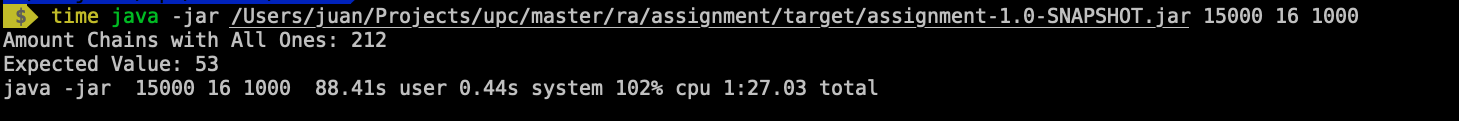
\includegraphics[width=\textwidth]{experiment6}
  \captionof{figure}{Expriment with n=15000}
  \label{fig:experiment6}
\end{minipage}

\subsection{$|S_n| = 20000$}

\begin{minipage}[t]{\linewidth}
  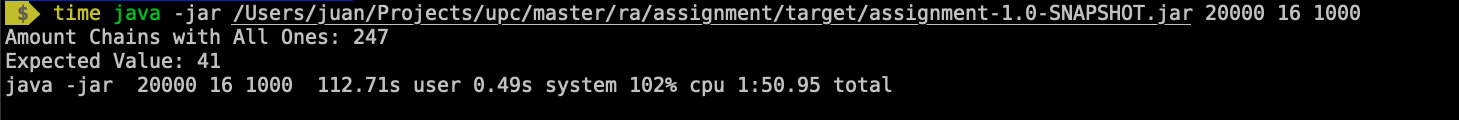
\includegraphics[width=\textwidth]{experiment7}
  \captionof{figure}{Expriment with n=20000}
  \label{fig:experiment7}
\end{minipage}


\section{Analysis of the Experiments}\label{an:data}
We have verified that for obtaining the $E[M_n]$ we need to analyze and run
several experiments in order to get an accurate statistical significance value
avoiding the dispersion of the sample, as we are going to show next.

\begin{minipage}[t]{\linewidth}
\centering
\begin{tikzpicture}
  \begin{axis}
    [
    xlabel={$|S_n|$},
    ylabel={$E[M_n]$},
    xmin=500, xmax=20000,
    ymin=1, ymax=200,
    scaled x ticks = true,
    scaled y ticks = true,
    legend style={nodes=right},
    ]
    \addplot coordinates {
      (500, 134)
      (1500, 153)
      (3000, 137)
      (6000, 103)
      (10000, 76)
      (15000, 53)
      (20000, 41)
    };
  \end{axis}
\end{tikzpicture}
\captionof{figure}{Distribution of experiments. Relation between $|S_n|$ and $E[M_n]$}
\label{fig:dist1}
\end{minipage}


As we can see in the distribution of the experiments \ref{fig:dist1}, as long as
$n$ grows, the expected value decrease.

This can be explained seeing the screenshots on \ref{sec:exp}. As we can
appreciate there as long as $n$ grows it is also growing the number of samples
in which $MAX(S_n) = \text{all one's chain}$.

\begin{table}[h!]
  \begin{tabular}{ |c|c|c|c|  }
    \hline
    \multicolumn{4}{|c|}{Experiment Table} \\
    \hline
    $|S_n|$ & $MAX(S_n) = \text{all one's chain}$ & $E[M_n]$ & $MAX(S_n) = \text{all one's chain}/E[M_n]$\\
    \hline
    500 & 4 & 134 & 0.03\\
    1500 & 16 & 153 & 0.10\\
    3000 & 35 & 137 & 0.25\\
    6000 & 96 & 103 & 0.93\\
    10000 & \color{red}{131} & 76 & 1.72\\
    15000 & \color{red}{212} & 53 & 4\\
    20000 & \color{red}{247} & 41 & 6.02\\
    \hline
  \end{tabular}
  \captionof{figure}{Relation between $|S_n|$, Chain with all one's, and $E[M_n]$}
  \label{table:relexp}
\end{table}

This is explaining why the Expected Value is decreasing as long as $|S_n|$
increasing. Since our samples is bigger when we increase $|S_n|$, the
probability of getting more chain with all ones increase. Therefore the median
is lower.

In this sense as we have seen in the lecture about \textbf{Concentration of a
  random variable around the mean}, we are getting extreme Values and therefore
the median does not show how $E[M_s]$ is concentrated in one value.

Taking into consideration the expressed before, we can also state that as long
as $|S_n|$ approximates the total Set $2^n$, in this case $2^16$, the expected
value with this method is not statistical significant.

\section{Conclusion}
In conclusion and accordingly on what we have stated before in \ref{an:data}, we
believe that in general for this experiment, taking into consideration only the \textbf{statistical significant samples}, the expected value has the following form:

\begin{equation}
  E[M_n] \sim \frac{\sqrt{2^n}}{2} 
\end{equation}

We have also checked that as long as $|S_n|$ grows, the number of \textbf{chains with
  all ones} also increase. This could be happening because of 2 reasons: First
because the population is bigger and therefore the $P[\text{all ones}]$ is not
so small as in other populations, and secondly because the Random generator to
toss the coin and generate the chain is a \textbf{build-in Java function} and it
could be a weak random generator for big populations. It is well know that there are other
more sophisticated \textbf{RNG} that simulates Randomness better, like \text{Composition by selection}.




\end{document}
